Si bien la base de datos Firebase Firestore proporciona una capa de conexión en tiempo real, es necesario introducir un nuevo método de comunicación permanente para notificar de eventos como lo son la presencia de usuarios activos y la visualización de las ordenes. Socket.IO permite la comunicación bidireccional entre el cliente y el servidor. Las comunicaciones bidireccionales se habilitan cuando un cliente tiene Socket.IO en el navegador, y un servidor también ha integrado el paquete. Si bien los datos se pueden enviar de varias formas, JSON es el más simple. Resume muchos tipos de transportes, incluidos \acrshort{ajax}  y WebSockets, en una sola API. Permite a los desarrolladores enviar y recibir datos sin preocuparse por la compatibilidad entre navegadores \cite{kelleher}.
\vspace{0.8cm}

En cualquier aplicación en tiempo real, mostrar múltiples usuarios en línea es muy importante, esta información debe actualizarse cuando un nuevo usuario se conecta o un usuario en línea se desconecta.
\vspace{0.8cm}

\begin{figure}[H]
  \centering
  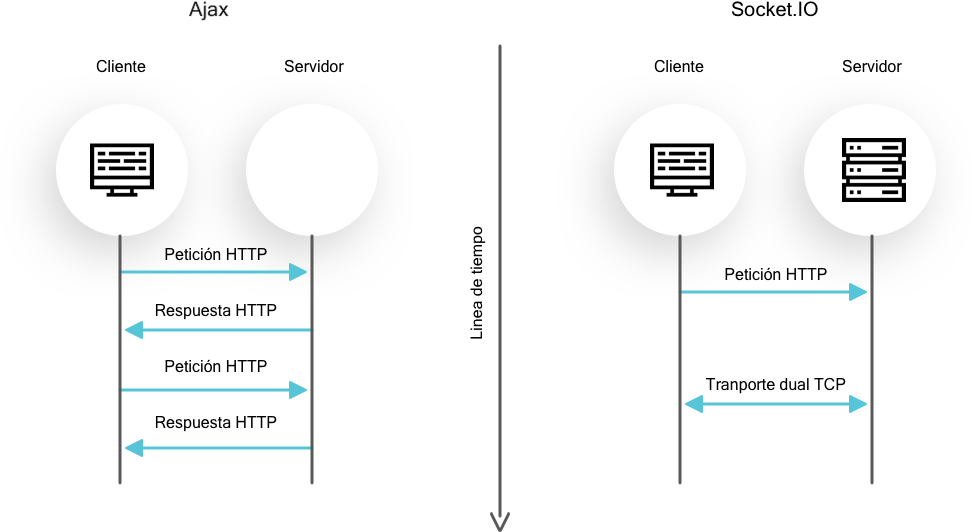
\includegraphics[width=1\textwidth]{websocket}
  \caption{Comparación de transporte por sondeo (Ajax) y websockets (Socket.IO).}
\end{figure}

\lstinputlisting[style=ES6, caption=Fragmento de configuración de Socket.IO del sistema]{code/socket.js}